\documentclass{beamer}
\usepackage{graphicx}
\usepackage{soul}
\usepackage{subcaption}
\usepackage{multicol}

\newcommand{\heading}[1]{{\Large\bfseries #1}\vspace{1em}}

\usetheme{CambridgeUS}

\title[Voting Sytems]{The Mathematics of Voting Systems}
\subtitle{Arrow's Theorem}
\author{Dylan Nelson}
\institute[SUMS]{Stellenbosch University Mathematics Society}
\date{1 October 2020}

\AtBeginSection[]{
    \begin{frame}
        \frametitle{Outline}
        \begin{multicols}{2}
            \tableofcontents[currentsection]
        \end{multicols}
    \end{frame}
}

\begin{document}
    \frame{\titlepage}

    \begin{frame}
        \frametitle{Outline}
        \begin{multicols}{2}
            \tableofcontents
        \end{multicols}
    \end{frame}

    \section{Play Along At Home}
    \begin{frame}
        \frametitle{Participate in our Mock Election}
    
        A survey is available at \url{https://www.surveymonkey.com/r/62WLLV9} where you can rank some ``integers'' in order of preference.

        \begin{center}
            
\includegraphics[width=0.3\linewidth]{surveymonkey_qr_code.png}
        \end{center}

        Later in the talk, a top secret method will be used to combine everyone's rankings into one overall ranking.
    
    \end{frame}

    \section{Addressing the Clickbait}
    \begin{frame}
        \frametitle{Clickbait}
    
        Some of you may have noticed that the poster advertising this talk is a bit clickbaity.

        \begin{center}
            
\includegraphics[width=0.5\linewidth]{poster.jpeg}
        \end{center}
    
    \end{frame}
    \begin{frame}
        \frametitle{Betteridge's Law of Headlines}
    
        \begin{block}{Betteridge's Law of Headlines}
            Any headline that ends in a question mark can be answered by the word ``no''.
        \end{block} 

        \begin{itemize}
            \item Betteridge's Law of Headlines may apply! \pause
            \item There is a Twitter account dedicated to this premise that has unfortunately been inactive since 2015: @YourTitleSucks.
        \end{itemize}

    \end{frame}
    \begin{frame}
        \frametitle{@YourTitleSucks}
    
        \begin{center}
            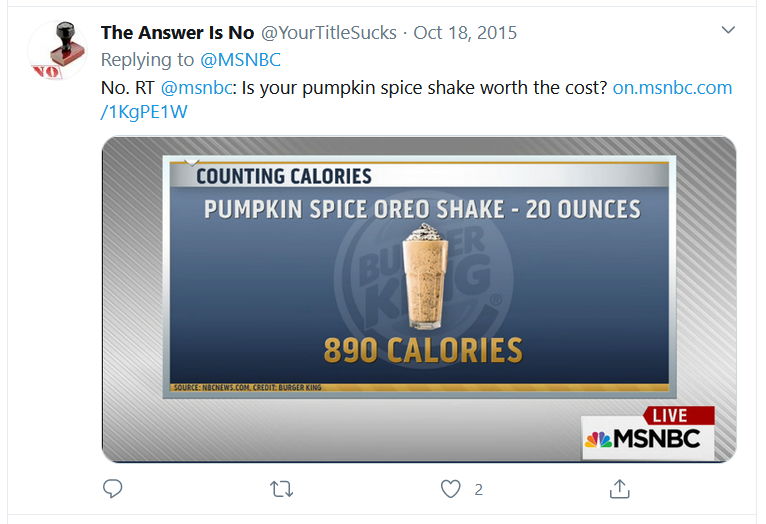
\includegraphics[width=0.8\linewidth]{pumpkin_spice.png}
        \end{center}
    
    \end{frame}
    \begin{frame}
        \frametitle{@YourTitleSucks}
    
        \begin{center}
            
\includegraphics[width=0.8\linewidth]{ufo.png}
        \end{center}
    
    \end{frame}
    \begin{frame}
        \frametitle{@YourTitleSucks}
    
        \begin{center}
            
\includegraphics[width=0.8\linewidth]{true_love.png}
        \end{center}
    
    \end{frame}
    \begin{frame}
        \frametitle{@YourTitleSucks}
    
        \begin{center}
            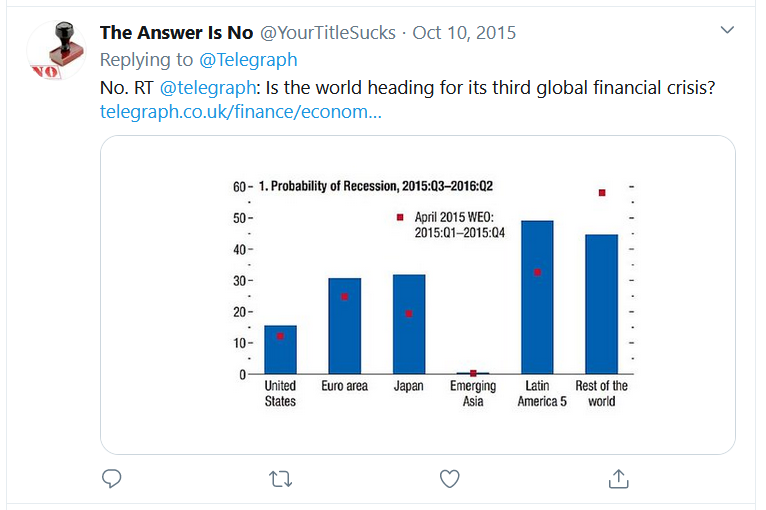
\includegraphics[width=0.8\linewidth]{crisis.png}
        \end{center}
    
    \end{frame}

    \section{Disclaimer}
    \begin{frame}
        \frametitle{Disclaimer}

        Last time I gave this talk, it was suggested that I not use actual political party names so as not to make the talk too political, but I didn't listen. I'll try to do better this time.
    
        \begin{block}{Disclaimer}
            Political parties referenced in this talk are either the product of the author's imagination or used in a fictitious manner. Any resemblance to actual political parties, local or abroad, or actual events, ideological positions, or policies is purely coincidental .
        \end{block}

    \end{frame}

    \section{Ranked List Voting Systems}
    \begin{frame}
        \frametitle{Ranked List Voting System}
    
        \begin{itemize}
            \item The systems that we will be considering require the voters to rank all of the candidates in order of preference rather than picking a single candidate to vote for.
            \item The goal of the system will be to combine these individual rankings into one overall ranking of all of the candidates.
        \end{itemize}
    
    \end{frame}
    
    \section{Desirable Properties for a Ranked List Voting System}
    \begin{frame}
        \frametitle{Determinism}

        \begin{itemize}
            \item The output of the system should only depend on the individual rankings provided by the voters.\pause
            \item If we have two different elections, and every voter gives the same ranking of the candidates in each election, then the output for the two elections should be the same. \pause
            \item We can't, for example, pick the winner based on what the weather is like.
        \end{itemize}

    \end{frame}
    \begin{frame}
        \frametitle{Universality}
    
        \begin{itemize}
            \item Every possible set of rankings provided by the voters should be accounted for.\pause

            \item It would also be nice if every possible ranking of the candidates could be obtained as an overall result. For example, if every voter gave that ranking as their preference, then it makes sense for that to be the overall result. But this isn't strictly necessary.\pause
        \end{itemize}

        \begin{block}{Remark}
            The properties of \alert{Determinism} and \alert{Universality} are really just saying that our aggregation system should be a (surjective) function from the space of possible elections to the space of possible rankings of the candidates.
        \end{block}
    
    \end{frame}
    \begin{frame}
        \frametitle{Unanimity}
    
        \begin{itemize}
            \item If \alert{every} voter prefers candidate A to candidate B, the the voting system should rank candidate A above candidate B overall.
        \end{itemize}

    \end{frame}
    \begin{frame}
        \frametitle{Independence of Irrelevant Alternatives (IIA)}
    
        \begin{itemize}
            \item Suppose that we have two elections. Suppose that every voter who preferred the Vulture Party to the Hyena Party in the first election still preferred the Vulture Party to the Hyena Party in the second election, and vice versa. \pause

            \item Then if the voting system ranks the Vulture Party above the Hyena Party in the first election, it should still do so in the second election. Similarly, if the voting system ranks the Vulture Party below the Hyena Party in the first election, then it should still do so in the second election. \pause

            \item The relative rankings of two candidates should only depend on how each voter ranked those two candidates against to each other.
        \end{itemize}

    \end{frame}

    \section{Examples of Voting Systems}
    \subsection{Two Candidates}
    \begin{frame}
        \frametitle{Two Candidates}
    
        \begin{itemize}
            \item Suppose that we only have two candidates, the Leech Party, and the Vulture Party.
            \item We count how many voters rank the Leeches above the Vultures, and vice-versa.
            \item If more voters prefer the Leeches to the Vultures than vice-versa, we rank the Leeches above the Vultures.
            \item Otherwise we rank the Vultures above the Leeches.
        \end{itemize}
    
    \end{frame}
    \begin{frame}
        \frametitle{Two Candidates}
    
        \begin{description}
            \item[Unanimity] If every voter prefers the Leeches to the Vultures, then certainly more voters prefer the Leeches to the Vultures than vice-versa, and so we rank the Leeches above the Vultures. \pause
            \item[IIA] Suppose we have two elections. If the relative rankings of the Leeches and the Vultures doesn't change between these two elections, then the candidate that is preferred more often also doesn't change, and so the result doesn't change.
        \end{description}
    
    \end{frame}

    \subsection{Positional Voting}
    \begin{frame}
        \frametitle{Positional Voting}
    
        \begin{itemize}
            \item For each candidate, we keep track of an overall score. \pause
            \item Every time the candidate is ranked $n^\text{th}$, we increase their score by $n$. \pause
            \item We then rank the candidates from the lowest score to the highest score. \pause
            \item To make the system deterministic/universal, we must choose a deterministic method to break ties. e.g. Alphabetically.
        \end{itemize}
    
    \end{frame}
    \begin{frame}
        \frametitle{Positional Voting}
    
        \heading{Unanimity}

        Suppose that voter $i$ ranks the Hyena Party in position $H_i$, and the Vulture Party in position $V_i$. \pause

        If every voter prefers the Hyena Party to the Vulture Party, then $H_i < V_i$ for all $i$. \pause

        Thus
        \[
            \text{Score for Hyena Party} = \sum H_i < \sum V_i = \text{Score for Vulture Party}
        \] \pause
    
        The system thus ranks the Hyena Party above the Vulture Party.
    \end{frame}
    \begin{frame}
        \frametitle{Positional Voting}
    
        \heading{IIA}

        Consider the following elections between the candidates H, V, L, and A:
        
        \begin{center}
            \begin{tabular}{|c|c|c|}
                \hline
                Voter & Election 1 & Election 2 \\
                \hline
                1 & H V A L & H A V L \\
                2 & L V H A & L H A V \\
                \hline
            \end{tabular}
        \end{center} \pause

        In the first election, V has $4$ points and so is ranked above L which has $5$ points. (Regardless of how the tie is broken between H and V) \pause

        In the second election, V has $7$ points and so is ranked below L which has $5$ points. \pause

        \alert{But} every voter who preferred H to V in the first election still did in the second election and vice-versa. \pause

        Thus \emph{Positional Voting} \alert{does not satisfy} IIA!
    
    \end{frame}
    \begin{frame}
        \frametitle{Positional Voting}
    
        \begin{center}
            
\includegraphics[width=0.5\linewidth]{disappointed_emoji.png}
        \end{center}
    
    \end{frame}

    \subsection{Copeland's Method}
    \begin{frame}
        \frametitle{Copeland's Method}
    
        \begin{itemize}
            \item For each pair of candidates, we pretend that the election is only between those two candidates and see who wins according to the Two Candidate method. \pause
            \item For each candidate, we count how many of these virtual elections they win and how many they lose. \pause
            \item The candidate's score is then the number of victories minus the number of defeats. \pause
            \item Copeland's Method is guaranteed to find a \emph{Condorcet Winner} if one exists.
        \end{itemize}
    
    \end{frame}
    \begin{frame}
        \frametitle{Condorcet Winner}
    
        \begin{block}{Definition}
            A \emph{Condorcet Winner} is a candidate that would beat any of the other candidates if we were to hold a head-to-head election between the two candidates.
        \end{block}
    
    \end{frame}
    \begin{frame}
        \frametitle{Copeland's Method}
        \heading{Unanimity}

        \begin{itemize}
            \item If every voter prefers A to B, then every time B beats a candidate in a sub-election, so does A. Thus the number of times that A wins a sub-election is at least as large as the number of times that B wins. \pause
            \item Similarly, A has at most as many defeats as B does.
            \item In particular, A beats B in the sub-election between A and B, and so in fact A has strictly more victories and strictly fewer defeats than B.
            \item The score assigned to A is thus larger than that assigned to B, and so Copeland's Method ranks A above B.
        \end{itemize}
    
    \end{frame}
    \begin{frame}
        \frametitle{Copeland's Method}
        \heading{IIA}

        Consider the following elections:
        \begin{center}
            \begin{tabular}{|c|c|c|}
                \hline
                Voter & Election 1 & Election 2 \\
                \hline
                1 & A B C D & A D B C \\
                2 & A C B D & A D C B \\
                3, 4 & B D A C & D B A C \\
                5, 6 & C D A B & D C A B \\
                \hline
            \end{tabular}
        \end{center} \pause

        In the first election, A is ranked above D, while in the second election, D is ranked above A. \pause

        \alert{But} every voter who preferred A to D in the first election still did in the second election, and vice-versa. \pause

        Thus \emph{Copeland's Method} \alert{does not satisfy} IIA!
    
    \end{frame}
    \begin{frame}
        \frametitle{Copeland's Method}
    
        \begin{center}
            
\includegraphics[width=0.6\linewidth]{sigh.png}
        \end{center}
    
    \end{frame}

    \subsection{Run-off Voting}
    \begin{frame}
        \frametitle{Run-off Voting}
    
        \begin{itemize}
            \item For each candidate, we count how many times they are the \emph{first choice} of some voter. \pause
            \item The candidate that is ranked first the fewest number of times is ranked last, and is eliminated from further consideration. \pause
            \item We then count how many times each remaining candidate is ranked above all of the remaining candidates by some voter. \pause
            \item The candidate that is ranked first among the remaining candidates the least number of times is ranked second-last, and eliminated from further consideration. \pause
            \item We continue in this manner until no candidates remain.
        \end{itemize}
    
    \end{frame}
    \begin{frame}
        \frametitle{Run-off Voting}
    
        \begin{itemize}
            \item The South African parliament uses a version of run-off voting to elect the President of South Africa. The President is \alert{not} necessarily the leader of the largest political party, and is not elected directly by the people of South Africa. \pause
            \item Any of member of Parliament can nominate any other member of Parliament to stand for President. \pause
            \item All of the members of Parliament then vote for one of the nominated candidates. \pause
            \item If any of the candidates have more than $50\%$ of the votes, then they become the President.
        \end{itemize}
    
    \end{frame}
    \begin{frame}
        \frametitle{Run-off voting}
    
        \begin{itemize}
            \item If no candidate wins the first round of voting, the candidate with the fewest number of votes is eliminated, and every member of Parliament votes again. \pause
            \item Note that unlike in the version of run-off voting we looked at, the members can change their vote at this point. \pause
            \item This process continues until one of the candidates has a majority. \pause
            \item Thus far only one round of voting has ever been necessary because our largest political party has always had a majority in Parliament.
        \end{itemize}
    
    \end{frame}
    \begin{frame}
        \frametitle{Run-off voting}
        \heading{Unanimity}
    
        If every voter prefers candidate A to candidate B, then A will always be the first remaining choice at least as often as B is. (In fact B is never ranked first as long as A has not been eliminated.) \pause

        Thus B will be the least popular candidate before A is, and so B is eliminated before A is. \pause

        The voting system thus ranks A above B.

    \end{frame}
    \begin{frame}
        \frametitle{Run-off voting}
        \heading{IIA}
    
        Consider the following two elections:
        \begin{center}
            \begin{tabular}{|c|c|c|}
                \hline
                Voter & Election 1 & Election 2 \\
                \hline
                1, 2 & A B C & A B C \\
                3, 4 & C B A & B C A \\
                5 & B A C & B A C \\
                \hline
            \end{tabular}
        \end{center} \pause

        In the first election, the result is A C B, while in the second election, the result is B A C. \pause

        But every voter who preferred A to B in the first election still did in the second election, and vice-versa. \pause

        Thus \emph{Run-off Voting} \alert{does not satisfy} IIA!

    \end{frame}
    \begin{frame}
        \frametitle{Run-off Voting}
    
        \begin{center}
            
\includegraphics[width=0.4\linewidth]{got_to_be_kidding_me.jpg}
        \end{center}
    
    \end{frame}
    
    \subsection{Other Methods}
    \begin{frame}
        \frametitle{Other Methods}
    
        \begin{itemize}
            \item There are many other methods that exist for the purpose of or can be adapted for the purpose of aggregating a set of rankings into one unified ranking.
                \begin{itemize}
                    \item The Borda Count
                    \item The Ranked Pairs Voting Method
                    \item The Kerney-Young Method
                    \item And many, many more! 
                \end{itemize} \pause
            \item You might be surprised to hear that \emph{none of them} satisfy the IIA!
            \item Is there any method that does?
        \end{itemize}
    
    \end{frame}

    \subsection{Dictatorship!}
    \begin{frame}
        \frametitle{Dictatorship!}
    
        \begin{itemize}
            \item We designate one of the voters as our hopefully-benevolent \st{dictator} King or Queen. \pause
            \item The overall ranking is just whatever they decide it is.
        \end{itemize}
    
    \end{frame}
    \begin{frame}
        \frametitle{Dictatorship!}
        \heading{Unanimity}
    
        If every voter prefers the Hyena Party to the Leech Party, then so does the dictator. \pause

        A dictatorship would thus rank the Hyena Party above the Leech Party.

    \end{frame}
    \begin{frame}
        \frametitle{Dictatorship!}
        \heading{IIA}        
    
        Suppose that we have two elections, and every voter who prefers the Hyena Party to the Leech Party in the first election still does in the second election, and vice-versa. \pause

        If the dictator prefers the Hyena Party to the Leech Party in the first election, then the Hyena Party is ranked above the Leech Party in the first election. \pause

    \end{frame}
    \begin{frame}
        \frametitle{Dictatorship!}
        \heading{IIA}
    
        By assumption, every voter who prefers the Hyena Party to the Leech Party in the fist election still does in the second election, and hence so does the dictator. \pause

        Thus the Hyena Party is still ranked above the Leech Party in the second election! \pause

        Conversely, if the dictator prefers the Leech Party in both elections, then the Leech Party is ranked higher in both elections. \pause

        Thus \emph{a Dictatorship} \alert{does satisfy} IIA!
    
    \end{frame}

    \section{Arrow's Theorem}
    \begin{frame}
        \frametitle{Arrow's Theorem}
    
        \begin{block}{Arrow's Theorem}
            Suppose that we have an election system for an election that is between $3$ or more candidates. If the system satisfies \alert{Determinism}, \alert{Universality}, \alert{Unanimity}, and \alert{Independence of Irrelevant Alternatives}, then it must be a dictatorship.
        \end{block}
    
    \end{frame}
    \begin{frame}
        \frametitle{Proof of Arrow's Theorem}
    
        I do not have slides prepared with the proof of Arrow's Theorem. If there is enough time, and enough people are interested, then I will switch to using another application to provide the sketch.
    
    \end{frame}

    \section{Does it Matter?}
    \begin{frame}
        \frametitle{Does it Matter?}

        \begin{itemize}
            \item Arrow's Theorem only applies to ranked-choice voting systems. In the real world, more information may be available. \pause
            \item We usually have an opportunity to correct our mistakes. \pause
            \item An election between ``Yes'' and ``No'' only has two candidates :P \pause
            \item Is IIA even such a desirable property anyway? \pause
            \item In the real world, people's preferences for parties are correlated.
        \end{itemize}
     
    \end{frame}

    \section{Conclusion}
    \begin{frame}
        \frametitle{Conclusion}
    
        \begin{center}
            {\Large Thank you for listening!}
        \end{center}

        \begin{figure}
            \centering
            \begin{subfigure}{0.27\linewidth}
                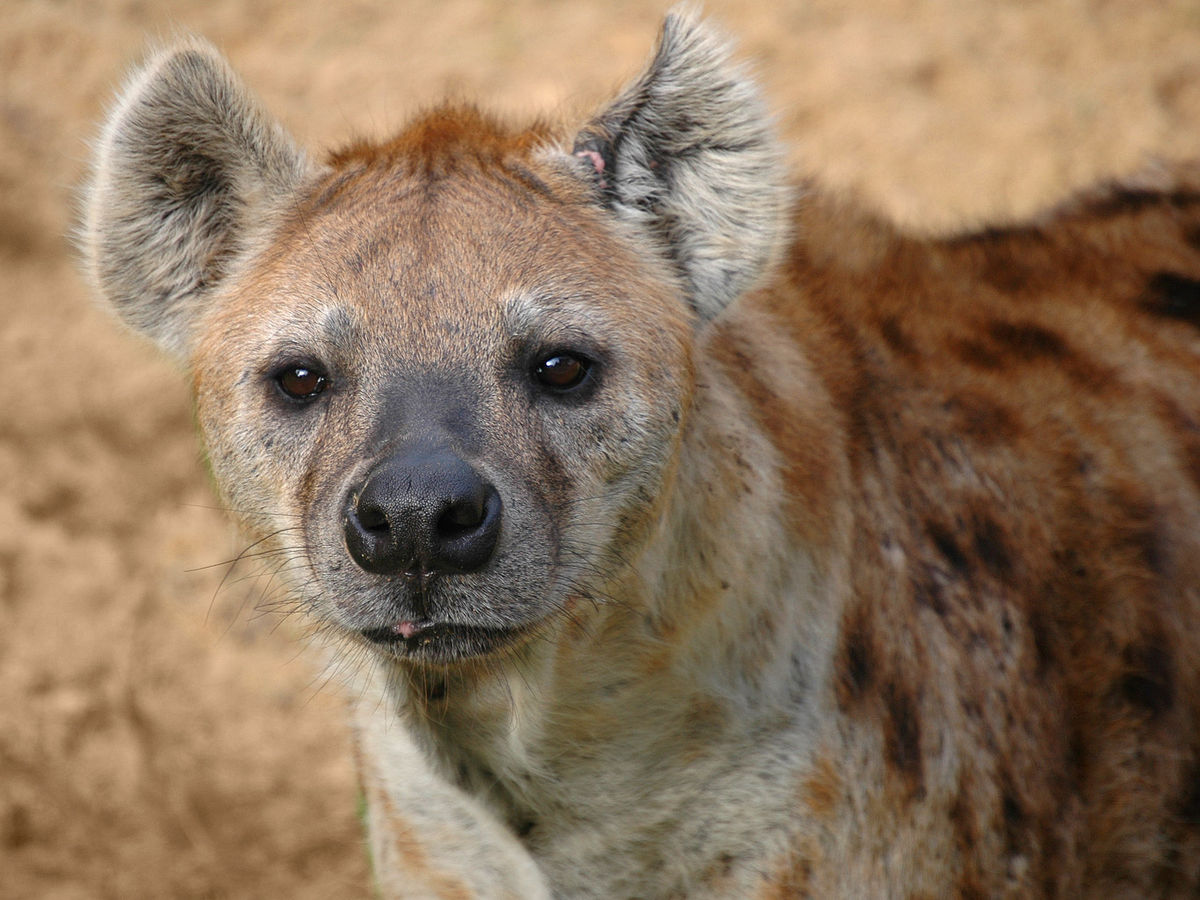
\includegraphics[width=\textwidth]{Hyena.jpg}
            \end{subfigure}
            \begin{subfigure}{0.32\linewidth}
                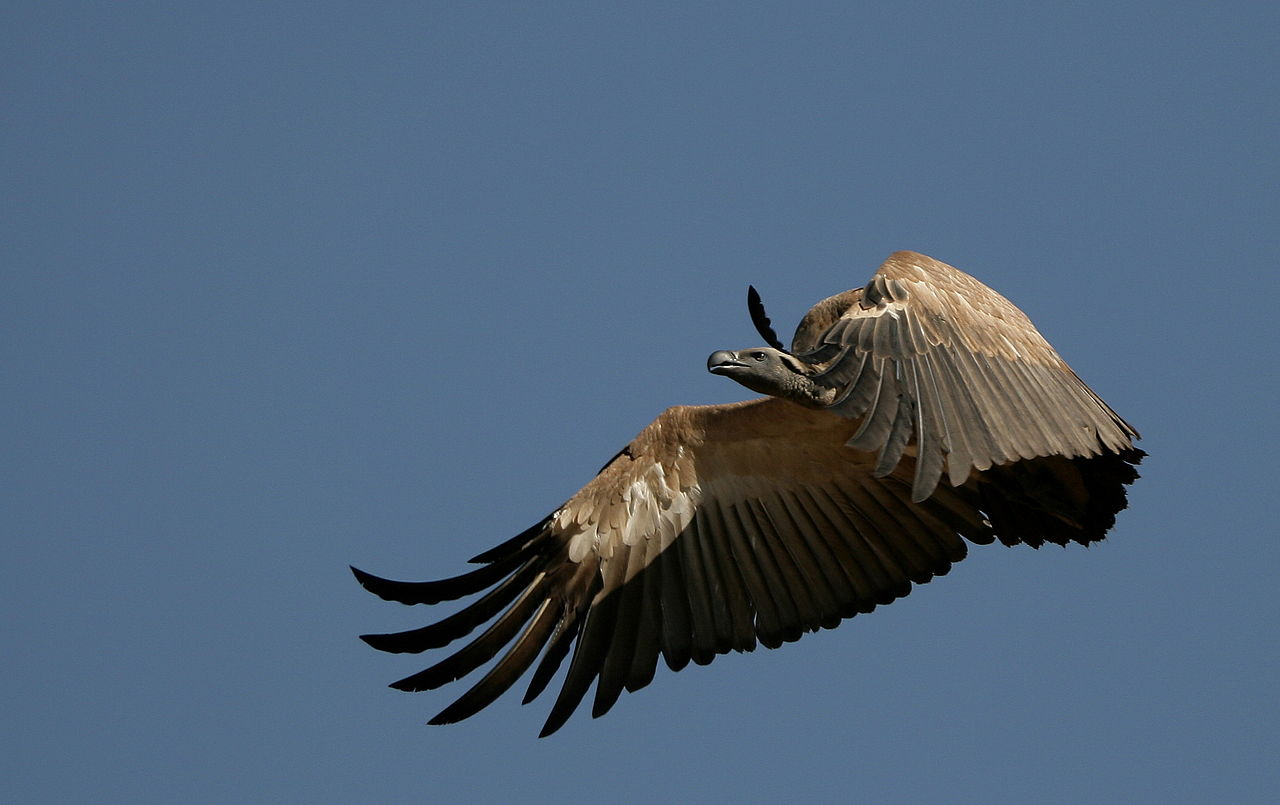
\includegraphics[width=\textwidth]{Vulture.jpg}
            \end{subfigure}
            \begin{subfigure}{0.27\linewidth}
                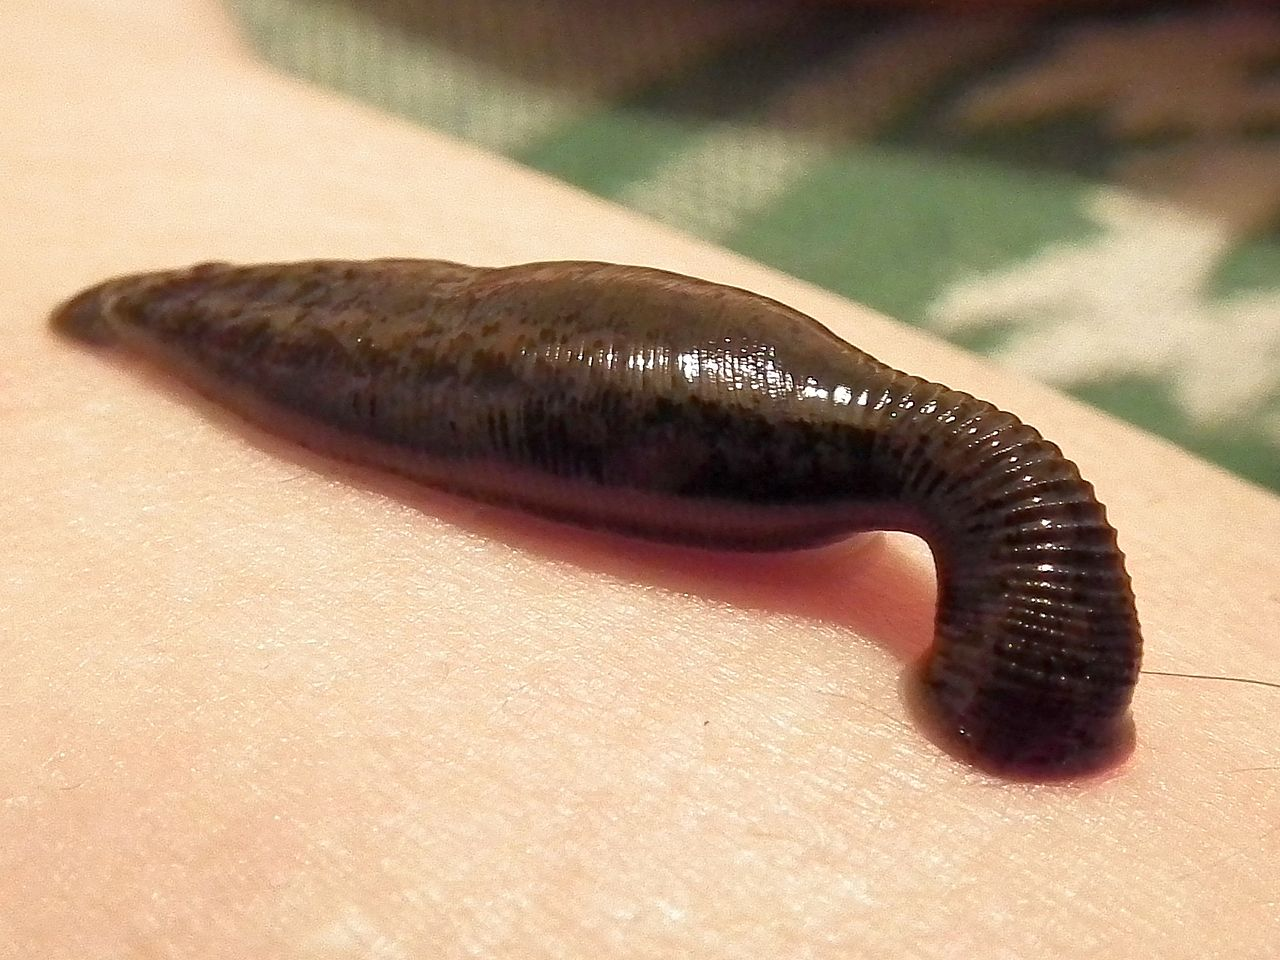
\includegraphics[width=\textwidth]{Leech.jpg}
            \end{subfigure}
        \end{figure}
    
    \end{frame}

\end{document}